\documentclass[a4paper, 15pt]{article}
\usepackage[left=0.85in, right=0.85in, top=0.5in, bottom=0.95in]{geometry}
\usepackage[T1]{fontenc}
\usepackage[utf8]{inputenc}
\usepackage[italian]{babel}

% Formattazione del testo
\usepackage{setspace}         % Setting dello spazio\begin{spacing}{0.95}
	\setstretch{1.2}
	\setlength{\parindent}{0pt}
	\raggedbottom
	\usepackage[none]{hyphenat}    % no sillabazione 
	\usepackage{multicol}          % testo su più colonne
	\usepackage{changepage, float}	       % \begin{adjustwidth}{}{}
		
		% Matematica
		\usepackage{amsmath, amssymb, amsthm, mathtools}
		\usepackage{cancel}            % semplificazioni \cancel{expression}
		\newtheorem*{thm}{Teorema}
		\newtheorem*{en}{Enunciato}
		\newtheorem*{definizione}{Definizione}
		\newtheorem*{cor}{Corollario}
		\DeclareMathOperator{\rk}{rk}
		\DeclareMathOperator{\im}{Im}
		
		% Simboli e Disegni
		\usepackage{color}             % \textcolor{'ColorCode'}{'testo'}
		\usepackage{graphicx, wrapfig}
		\usepackage{tikz, circuitikz}
		\usetikzlibrary{patterns, arrows, decorations.markings, arrows.meta, decorations.text}
		\tikzset{immagine/.style={above right, inner sep=0pt, outer sep=0pt},
			testo/.style={fill=white, align=center, fill opacity=0.6, text opacity=1, below, font=\sffamily\bfseries\footnotesize}}
		\usepackage{pgfplots}
		\pgfplotsset{compat=1.15}
		\usepackage{mathrsfs}
		
		% Altri pacchetti
		\usepackage{enumitem}
		\usepackage{mdwlist} 	       % suspend enumerate \suspend{} \resume{}
		\usepackage{siunitx}
		\usepackage{hyperref}
		\hypersetup{
			colorlinks=true,
			linkcolor=blue,    
			urlcolor=blue,
		}
		\urlstyle{same}
		
		% Altre definizioni personali
		\usepackage{pifont}
		\newcommand{\cmark}{\ding{51}}
		\newcommand{\xmark}{\ding{55}}
		\DeclareUnicodeCharacter{20AC}{\EUR}
		\newcommand{\compresslist}{\setlength{\itemsep}{1pt}\setlength{\parskip}{0pt}\setlength{\parsep}{0pt}}
		\newcommand{\ra}[1]{\renewcommand{\arraystretch}{#1}} % stretcho le tabelle e gli array \ra{x}
		\setlength{\jot}{10pt}
		
		
		% Titolo e data
		\title{Supporti}
		\date{}
		
		\begin{document}
			\maketitle
			\setcounterpageref{secnumdepth}{0}
			\setcounter{tocdepth}{5}  % Includo nel TOC anche i subsubpar	
			\tableofcontents 
			{\small \textit{Dagli appunti di Curzio Crociani}}
			\newpage
			
			\section{Cuscinetti}
			Il cuscinetto è un elemento funzionale che mi serve a sostenere l’albero e quindi limitarlo nei suoi spostamenti ma che garantisca il grado di labilità che l’albero contiene. \newline
			
			L’albero è un elemento labile perché è libero di ruotare attorno al proprio asse, il grado di libertà rotazione attorno al proprio asse è un grado di libertà che non bisogna in alcun modo vincolare perché è il grado di libertà attraverso il quale l’albero trasmette il moto e quindi trasmette il momento torcente. \newline 
			
			Quasi tutti i cuscinetti hanno molteplicità cinematica pari a 5 perché impediscono tutti gli spostamenti relativi e lasciano libera una rotazione relativa. \newline 
			
			Classifichiamo i cuscinetti in
			\begin{itemize}
				\item	\textbf{Cuscinetti Volenti} 
				
				Presentano degli elementi che si interpongono tra i due anelli del cuscinetto che rotolano, l’attrito quindi anziché essere un attrito di strisciamento (radente) è un attrito volvente che sappiamo avere un coefficiente d’attrito molto più basso rispetto all’attrito radente. \newline 
				
				Sono una soluzione estremamente affidabile e sono caratterizzati da una vita utile finita, la fatica prima o poi insorge sempre e porta alla sostituzione.
				Sono rumorosi perché presentano organi in rotazione.
				Hanno un ingombro assiale piccolo o comunque minore rispetto a quelli a strisciamento
				Hanno invece un ingombro radiale non trascurabile dato dalla presenza dei corpi volventi. \newline 
				
				Un grande svantaggio è quello di necessitare di un montaggio specifico in grado di prevedere il posizionamento e la registrazione della posizione. 
				
				
			\item 	\textbf{Cuscinetti a Strisciamento}
			
			In cui le due superfici almeno nella condizione iniziale strisciano l’una sull’altra, si instaurano poi delle condizioni di lavoro forzate o naturali per cui un lubrificante si interpone tra le parti che fa da meato di lubrificante in grado di garantire delle flessioni portanti sull’elemento sospeso tanto da tenerlo in posizione senza il contatto diretto. \newline 
			
			I cuscinetti a strisciamento più semplici detti anche Bronzine (perché realizzate in bronzo) sono semplicemente due cilindri cavi che vengono alloggiati e attraverso le caratteristiche di autolubrificazione del bronzo sono in grado di mantenere in posizione l’elemento.
			Il problema dei cuscinetti a strisciamento rispetto a quelli volventi è che hanno bisogno di una lubrificazione estremamente raffinata. \newline 
			
			Sono silenziosi e facili da montare.
			Una loro caratteristica importante è di resistere bene agli urti grazie anche al fatto che l’interposizione di un viscoso è fortemente smorzante. \newline 
			
			Utilizzati per alte velocità.
			Molto ingombranti assialmente ma poco ingombranti radialmente.
			Sono meno costosi rispetto ai cuscinetti volventi. 
			
			Sono in grado di sopportare carichi gravosi solo se sono in grado di garantirgli le condizioni di lubrificazioni idrodinamiche richieste. 
			
			
			\end{itemize}
			
			I cuscinetti sono elementi che soggetti ad usura e a fatica. 
			
			Ciò che accade in un cuscinetto dal punto di vista delle tensioni e dell’usura è molto complesso perché il contatto avviene in punti costantemente diversi; le pressioni hertziane di contatto tra i corpi saranno proprio la principale causa di usura e fatica. 
\newpage			
			\subsection{Tipi di cuscinetti volventi}
			\subsubsection{Cuscinetti radiali}
			Un cuscinetto volvente è formato da un anello esterno, un anello interno, una serie di corpi volventi che si interpongono (non vanno mai disegnati in sezione e vanno sempre rappresentati due corpi volventi a 180° l’uno dall’altro anche in caso il numero di corpi fosse dispari).
			\begin{figure}[H]
				\centering
				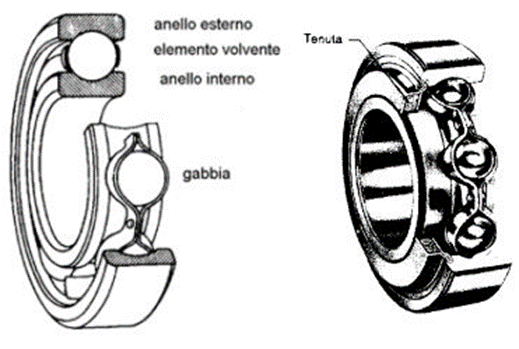
\includegraphics[width=0.5\linewidth]{immagini/screenshot001}
				\label{fig:screenshot001}
			\end{figure}
			Il corpo volvente può avere forme molto differenti tra loro:
			\begin{itemize}
			\item	Sfere
			\item	Rulli
			\item	Rulli conici (per garantire lo scarico delle forze in due direzioni, assiale e radiale)
			\item	Rulli a botte (soluzione utilizzata per avere cuscinetti orientabili)
			\item	Rullini (soluzione che garantisce poco ingombro radiale ma elevato ingombro assiale)
			\end{itemize}
			Sono in grado di ruotare anello interno e esterno relativamente di qualche grado così da compensare eventuali deformazioni dell’albero o errori di montaggio o eccessive tolleranze geometriche. \newline 
			
			Tutta la difficoltà ingegneristica sta nello studio dell’accoppiamento sfera – sede. 
			\begin{figure}[H]
				\centering
				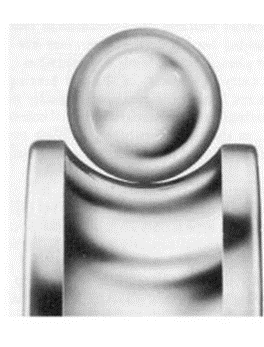
\includegraphics[width=0.25\linewidth]{immagini/screenshot002}
				\label{fig:screenshot002}
			\end{figure}
			Sarà infatti questo accoppiamento che genererà le forze, le pressioni hertziane, l’attrito e quindi le temperature che si instaurano.  \newline 
			
			In condizioni reali un contatto sfera-piano (sfera-sede) è un contatto puntuale che quindi genera una forza molto concentrata tendente a infinito (condizione ovviamente non fisica ma solo ideale) ma durante il funzionamento c’è uno schiacciamento relativo che porta delle deformazioni elastiche delle superfici che portano così ad estendere la superficie di contatto.
			
			\begin{itemize}
				\item Un perfetto compromesso tra l’estensione della deformazione e lo scarico delle forze mi permette di minimizzare gli effetti hertziani e di conseguenza le cause dei fenomeni di fatica.
				
				\item La forma della sede che non è perfettamente semicircolare ma ha una forma parabolica è tale da assorbire il più possibile i carichi radiali anche in presenza di deformazioni e spostamenti relativi della sfera. 
			\end{itemize}
			
			Per un certo valore di angoli di rotazione la sfera è ancora in grado di trasmettere il carico normalmente, superato però un certo limite la sede non è più in grado di trattenere le sfere e quindi si deformano sul bordo della sede e quindi il cuscinetto non lavora più in condizioni accettabili.
			
			\begin{figure}[H]
				\centering
				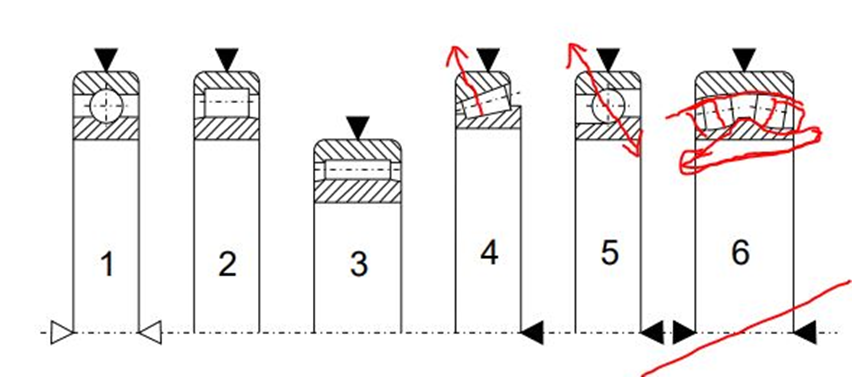
\includegraphics[width=0.5\linewidth]{immagini/screenshot003}
				\label{fig:screenshot003}
			\end{figure}
			\textbf{NB:} ogni volta che ho un trasferimento di carico tramite una superficie di contatto la direzione in cui trasferisco il carico è quella normale alla superficie di contatto.
			\begin{enumerate}
				\item \textbf{Cuscinetto radiale a sfere} 
				
				Consente principalmente di supportare un carico radiale ed un piccolo carico assiale.
				
				\item \textbf{Cuscinetti radiali a rulli}
				
				Lavorano radialmente, questo perché l’anello interno di solito presenta dei denti che trattengano il rullo e assialmente questo si può sfilare.
				
				\item \textbf{	Cuscinetti radiali a rullini }
				
				\item \textbf{	Cuscinetti obliqui a rulli conici }
				
				hanno un asse di rotazione inclinato rispetto all’asse di rotazione dell’albero. In questo modo il carico viene trasferito dall’albero verso la cassa in due direzioni una assiale e una radiale entrambi elevati.
				
				\item \textbf{Cuscinetti obliqui a sfere }
				
				Questi sono cuscinetti a sfere dove cambia la sede: dato che anche in questo caso la spinta è obliqua, anch’esso ha bisogno di un cuscinetto gemello orientato nella direzione opposta.
				
				\item \textbf{Cuscinetti a doppia corona di rulli a botte }
				
				I rulli a botte sono dei rulli che hanno una superficie di contatto non cilindrica ma leggermente bombata. Questa superficie mi permette di generare una sede di contatto a doppia curvatura. 
				
				Questi cuscinetti resistono a condizioni molto più estreme di deformazione dell’albero o talvolta in fase iniziale di montaggio sopperiscono a problemi geometrici di assemblaggio.
			\end{enumerate}
			\newpage			
			\subsubsection{Cuscinetti assiali, reggispinta}

			Tutti quei cuscinetti che supportano principalmente il carico assiale sono chiamati Cuscinetti Assiali o Reggispinta.
			\begin{figure}[H]
				\centering
				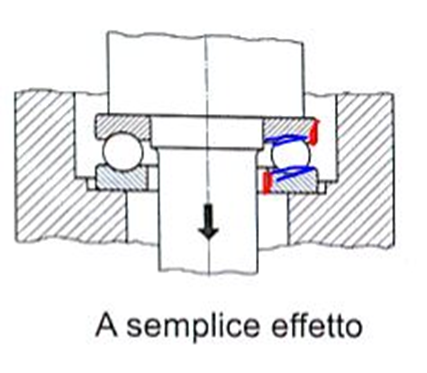
\includegraphics[width=0.25\linewidth]{immagini/screenshot004}
				\label{fig:screenshot004}
			\end{figure}
			Si catalogano rispettivamente in 
			\begin{itemize}
				\item A semplice effetto: sopportano il carico in una direzione;
				\item A doppio effetto: sopportano il carico in due direzioni. 
			\end{itemize}
			\begin{figure}[H]
				\centering
				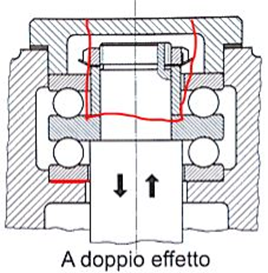
\includegraphics[width=0.25\linewidth]{immagini/screenshot005}
				\label{fig:screenshot005}
			\end{figure}
						
			Tutte quelle soluzioni che prevedono un avanzamento assiale regolabile mi consentono di avvicinare con la ghiera il cuscinetto fino alla posizione e quando arrivo alla posizione blocco il dentello della rosetta facendo rimanere in posizione il cuscinetto. 
			
			\begin{figure} [H]
				\centering
				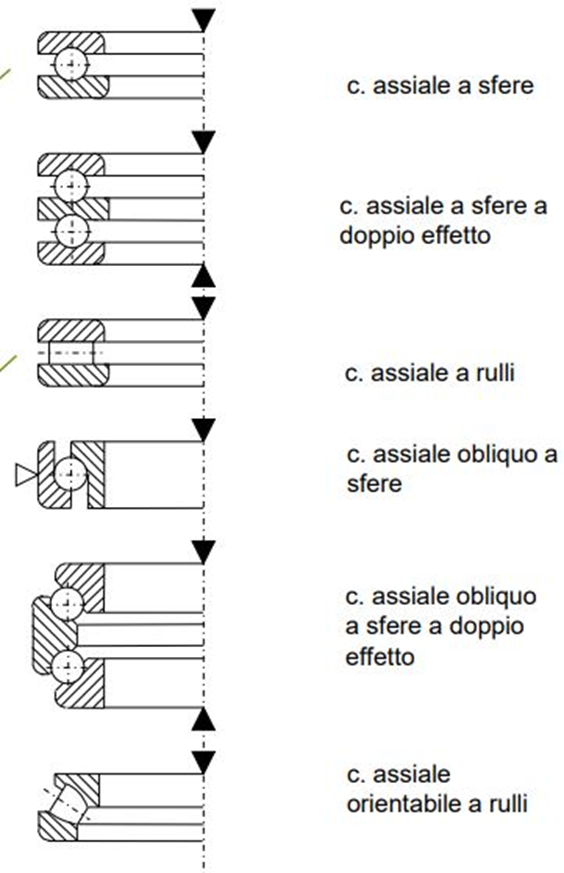
\includegraphics[width=0.25\linewidth]{immagini/screenshot006}
				\label{fig:screenshot006}
			\end{figure} 
			
			Le soluzioni \textbf{semiaperte} presentano un dentello anche nell’altra sede e consentono di supportare deboli carichi assiali in una direzione. 
			
			Nelle soluzioni \textbf{chiuse} si realizza nella sede inferiore un dentello come nelle soluzioni semiaperte e poi si inserisce una ghiera che ne blocca le sedi.
			
			
			\begin{figure}[H]				
\centering
				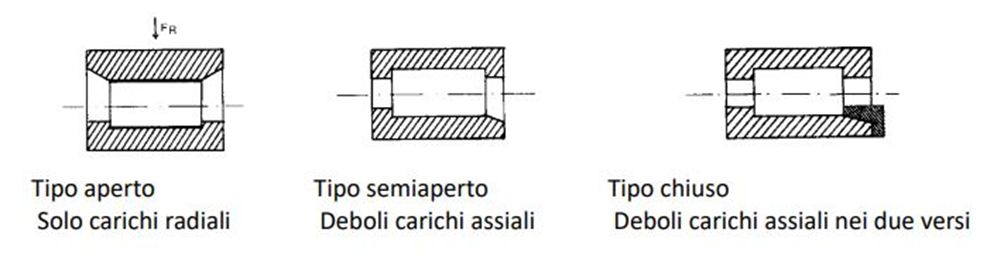
\includegraphics[width=0.5\linewidth]{immagini/screenshot007}
				\label{fig:screenshot007}

			\end{figure}
			
			
			\section{Montaggio}
			
			All’interno delle condizioni di montaggio devo fare molta attenzione al discorso termico.
			
			Dato che le dilatazioni termiche sono presenti in qualsiasi applicazione devo imparare a conviverci ovvero devo ridurre il più possibile gli effetti dal punto di vista delle tensioni delle dilatazioni termiche.
			
			\[\Delta L = \alpha\Delta TL\]
			
			La dilatazione termica è disaccoppiata nelle tre direzioni per cui nella direzione z dell’asse L è almeno 20 volte più dello spessore (ipotesi elemento snello), quindi la dilatazione assiale sarà almeno 20 volte superiore a quella in direzione radiale.
			
			Ci concentreremo perciò sulla dilatazione assiale.
			
			Tuttavia tale dilatazione non rende non-funzionale una ruota dentata: interesserà soltanto lo spostamento dei punti di calettamento di ruota e pignone. 
			
			Se il montaggio dell’albero è schematizzabile con uno schema cerniera carrello, quando l’albero viene riscaldato e si allunga dove trova libero spostamento - ovvero in corrispondenza del carrello- si dilaterà: la dilatazione termica si adatta, dove trova possibilità sfoga in quella direzione.\newline 
			
			Devo quindi garantire un montaggio isostatico perché io con le dilatazioni termiche ci posso convivere ma con gli stati tensionali derivanti dalle dilatazioni impedite no.
			
			
			\begin{center}
				\textbf{Tutto ciò che è in rotazione va in contatto esclusivamente con elementi in rotazione
					Tutto ciò che è fermo va in contatto solo con elementi fermi}
			\end{center}

				\begin{figure}[H]
		\centering
		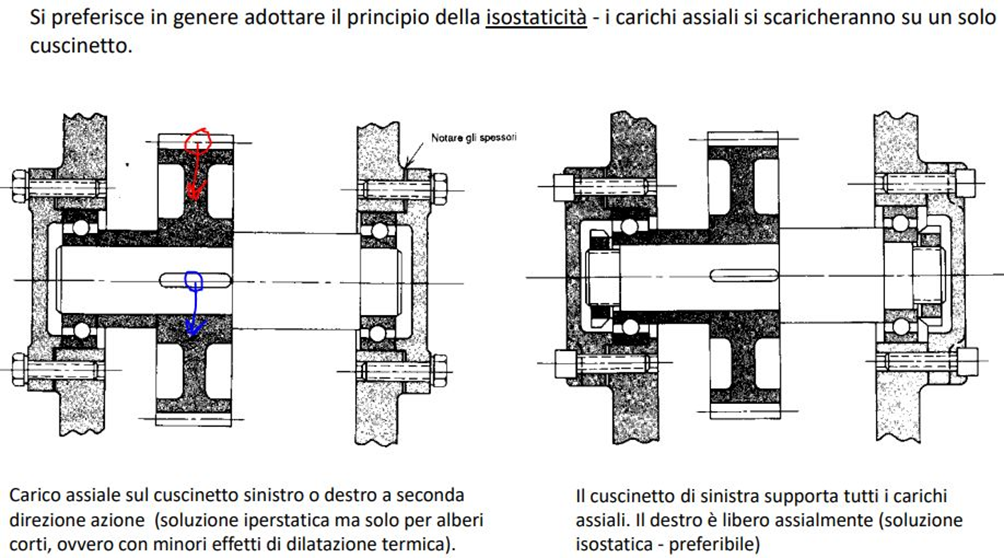
\includegraphics[width=0.5\linewidth]{immagini/screenshot008}
		\label{fig:screenshot008}
	\end{figure}
	
		\begin{figure} [H]
		\centering
		
		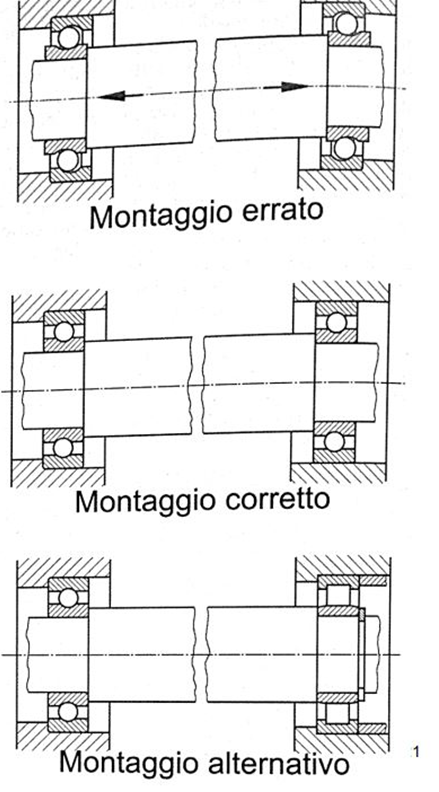
\includegraphics[width=0.25\linewidth]{immagini/screenshot009}
		\label{fig:screenshot009}
	\end{figure}
			Il \textbf{primo} montaggio è errato poiché in caso di dilatazioni termiche l’albero non è libero di allungarsi poiché l’anello esterno del cuscinetto è bloccato.
			
			Il \textbf{secondo} montaggio (anche se incompleto perché manca un sistema di arresto assiale dei cuscinetti) è corretto.
			
			Una soluzione \textbf{alternativa} può essere quella che prevede l’utilizzo di cuscinetti a rulli poiché come abbiamo visto questi cuscinetti per poter inserire i rulli hanno una delle due sedi completamente liscia che può essere sfruttata per ottenere lo scorrimento relativo.
			
			\begin{figure}[H]
				\centering
				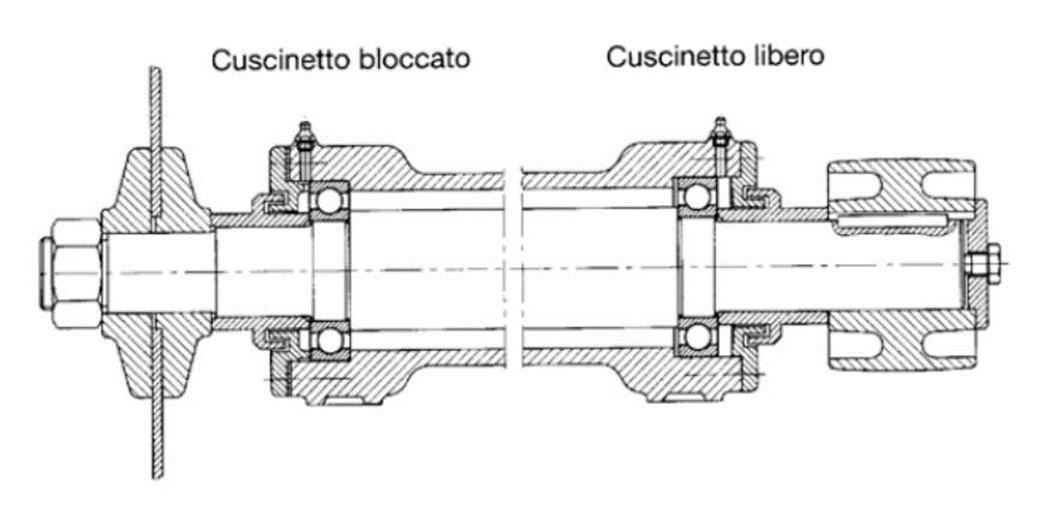
\includegraphics[width=0.5\linewidth]{immagini/screenshot010}
				\label{fig:screenshot010}
			\end{figure}
			In questo caso a \textbf{sinistra} l’anello interno è bloccato a destra dallo spallamento e a sinistra da un distanziale che è bloccato assialmente da un mozzo tenuto fermo da un dado avvitato sul codolo dell’albero (la parte finale filettata di un albero si chiama codolo) e anche l’anello esterno risulta bloccato.
			
			Nel cuscinetto a \textbf{destra} l’anello interno è bloccato nella stessa maniera dell’anello interno del cuscinetto di sinistra mentre l’anello esterno non tocca direttamente l’elemento che invece blocca l’anello esterno del cuscinetto di destra per cui eventuali dilatazioni dell’albero lo fanno spostare verso destra mentre eventuali contrazioni lo fanno spostare verso sinistra.
			\newpage
			\begin{figure}[H]
				\centering
				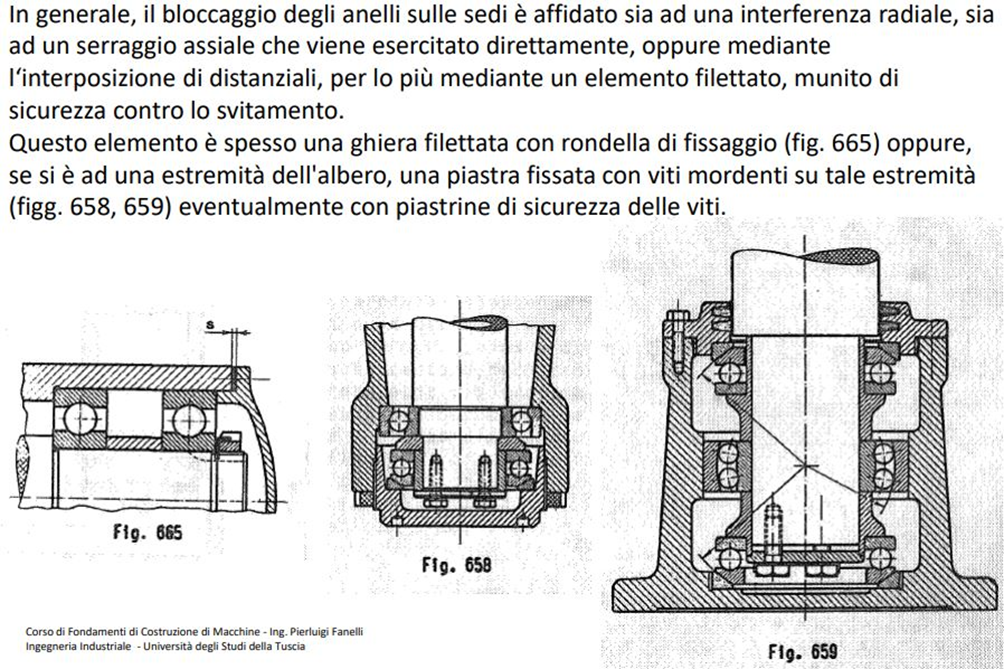
\includegraphics[width=0.5\linewidth]{immagini/screenshot011}
				\label{fig:screenshot011}
			\end{figure}
			Nella \textbf{terza figura} abbiamo un montaggio complesso iperstatico con due cuscinetti assiali a sfere e un cuscinetto a doppia sfera senza vincolo assiale. Questo montaggio è iperstatico ma dato che è di solito riservato alle parti terminali di un albero e quindi la distanza tra i cuscinetti è breve le dilatazioni termiche sono di un’entità accettabile e quindi questo montaggio anche se iperstatico è ammesso.
			\begin{figure}[H]
				\centering
				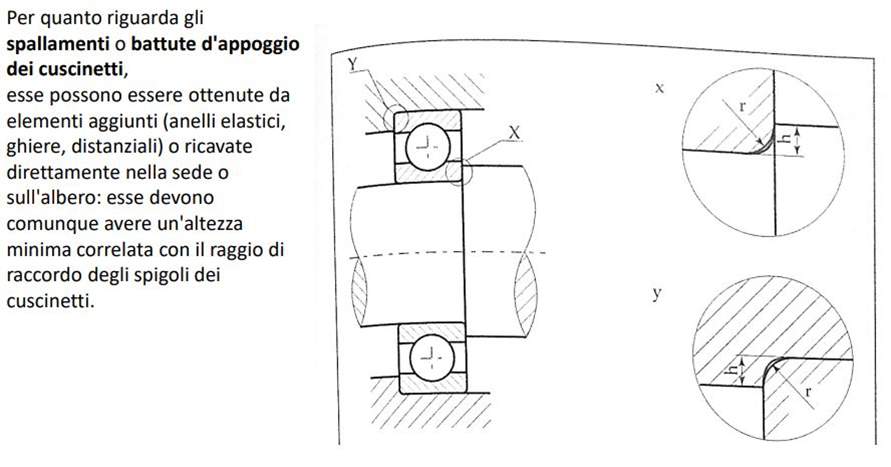
\includegraphics[width=0.5\linewidth]{immagini/screenshot012}
				\label{fig:screenshot012}
			\end{figure}
			
			\begin{center}
				\textbf{Il cuscinetto si monta nella parte serrata con un leggero forzamento mentre per il lato che deve scorrere utilizzo un accoppiamento incerto.}
			\end{center}
			
			Quando per una serie di motivi che sono ad esempio la nascita di forti carichi assiali ho la necessità di lavorare con dei cuscinetti obliqui allora questi devono essere sempre montati a coppia con direzione opposta della spinta per evitare che si smontino.
			\begin{figure}[H]
				\centering
				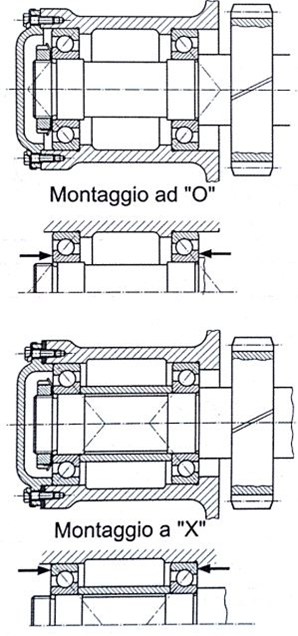
\includegraphics[width=0.15\linewidth]{immagini/screenshot013}
				\label{fig:screenshot013}
			\end{figure}
			
			\begin{itemize}
				\item Montaggio ad "O" per cassa rotante;
				\item Montaggio ad "X" per albero rotante.
			\end{itemize}
			
			Questo montaggio è intrinsecamente un montaggio iperstatico perché quel tratto di albero compreso fra i cuscinetti non può dilatare in nessun modo, o meglio, nel caso di montaggio ad O se dilata perdiamo la registrazione del cuscinetto mentre nel caso di montaggio ad X la dilatazione è impedita e viceversa la contrazione.  
\newpage			
			\begin{center}
				\textbf{Un cuscinetto assiale deve avere completa libertà radiale.}
			\end{center}
			
			\begin{figure}[H]
				\centering
				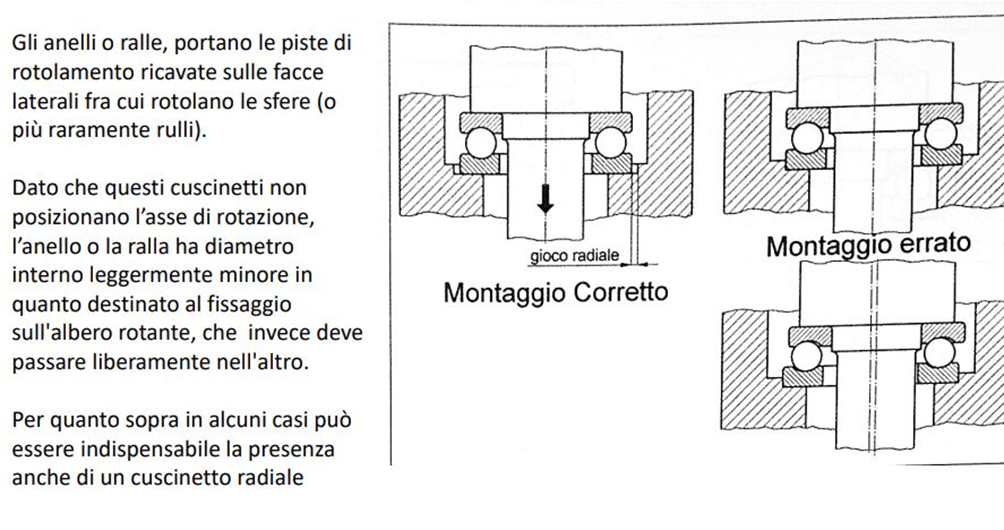
\includegraphics[width=0.5\linewidth]{immagini/screenshot014}
				\label{fig:screenshot014}
			\end{figure}
			
			\section{Resistenza}
			La resistenza del cuscinetto e la sua durata a fatica dipenderanno:
			\begin{itemize}
				\item	Dalle condizioni di contatto dei corpi volventi sulle piste
			\item	Dal ciclo di fatica agente e quindi dalla resistenza a contatto dei componenti
			\item	Una serie di altri parametri quali temperatura, lubrificazione, presenza di impurità\dots
			\end{itemize}
			
			\subsection{Studio del contatto}
			La resistenza di un cuscinetto è incentrata sul concetto di resistenza di contatto.
			
			E’ il contatto fra le parti in rotazione relativa che causa concentrazioni di tensioni e quindi l’insorgere di danneggiamenti. \newline
			
			Questo perché il contatto idealmente puntuale di una sfera su un piano genererà sempre una deformazione localizzata che porta ad avere nella realtà una superficie di contatto e quindi un’estensione della zona sollecitata alla pressione che è variabile con l’entità del carico.
			
			Se chiamo $\delta$ l’ideale compenetrazione tra la sfera e la superficie, sarà pari ad una costante C per il carico P normale alla superficie elevato alla 2/3.
			\begin{figure}[H]
				\centering
				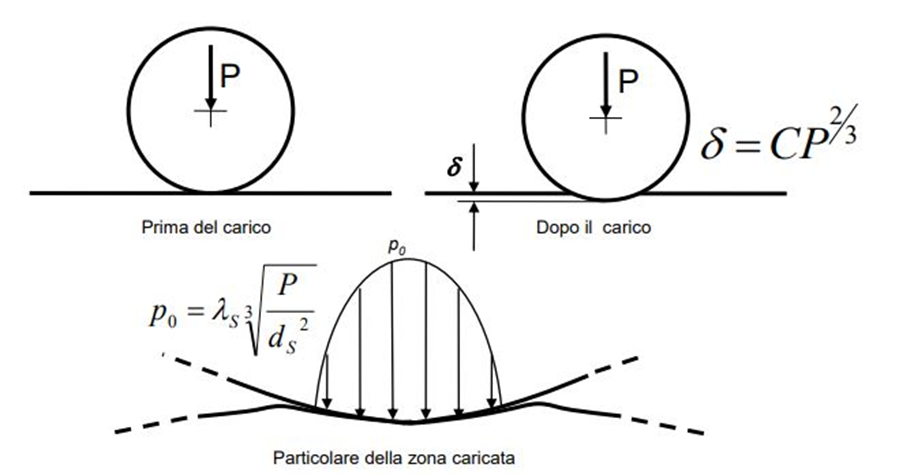
\includegraphics[width=0.8\linewidth]{immagini/screenshot015}
				\label{fig:screenshot015}
			\end{figure}
			Questa relazione che esprime delta deriva dalla formulazione della pressione hertziana, la quale ha un andamento parabolico, si estende lungo l’entità della superficie di contatto che però a sua volta è dettata dalla deformazione che si genera sulle due superfici (l’estensione di questa superficie di contatto dipende dalla deformazione localizzata) il cui valore massimo P0 di questo andamento parabolico si può sintetizzare con la relazione scritta sopra.
\newpage			
			\subsection{Analisi dei carichi sui corpi volventi}
			I corpi sono volventi: istante per istante un nuovo punto della sfera toccherà un nuovo punto della pista generando quindi una pressione hertziana che si sviluppa e si spegne in un punto in un certo intervallo di tempo. \newline
			
			In condizioni ideali la sommatoria di queste pressioni mi restituisce i carichi transitanti, naturalmente possibili disallineamenti, deformazioni, urti portano a constatare che lo stato tensionale nel tempo in un componente del cuscinetto è estremamente complesso da ricavare in dettaglio, si utilizzerà perciò il modello di \textbf{Stribeck}. 
			
			\begin{itemize}
				\item Corpi dal comportamento elastico lineare; 
				\item Effetti del contatto esclusivamente locali;
				\item Gli anelli subiscono delle deformazioni elastiche mantenendo globalmente la loro forma circolare. 
			\end{itemize}
			\begin{figure}[H]
				\centering
				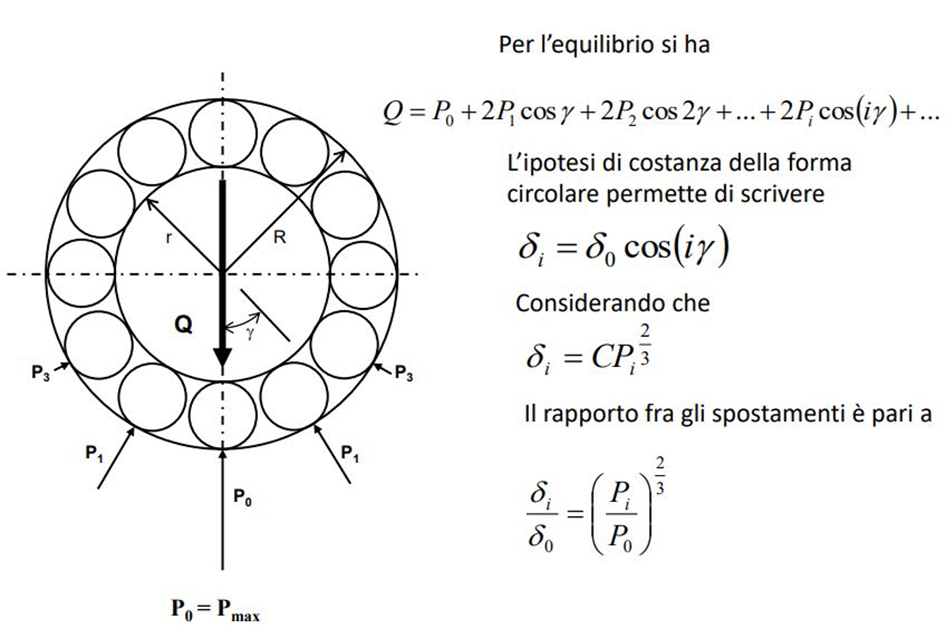
\includegraphics[width=0.8\linewidth]{immagini/screenshot016}
				\label{fig:screenshot016}
			\end{figure}
			Naturalmente il carico $Q$ è direzionato per cui avremo un set di sfere compresse e tutta una serie di sfere completamente oziose (scariche). 
			
			\begin{itemize}
				\item L’ipotesi forte di Stribeck - cioè quella per cui gli anelli rimangono circolari - mi porta a dire che quando applico il carico verso il basso sull’anello interno questo trasla verticalmente mantenendo la forma dove in realtà potrei avere una leggera ovalizzazione.\newline 
				
				Ciò vuol dire che imponendo tale spostamento rigido il carico si ripartisce con legge trigonometrica: la sfera direttamente sotto si prende tuttp $P_0 = P_{max}$; alle sfere affianco toccherà un carico $P_1$ minore e alle sfere più lontane un carico $P_i$ sempre decrescente.
				
				\item L’ipotesi sulla costanza della forma mi porta a dire poi che lo spostamento dell’anello, e quindi la compenetrazione $\delta_i$ di anello con sfera, è proporzionale a quello della sfera centrale $\delta_0$ perché è pur sempre generato da un cerchio: l’impronta che lascia sulle sfere sottostanti è proporzionale all’angolo.
			\end{itemize}
\newpage			
			Dall'equazione di equilibrio si ottiene così che il carico massimo sulla sfera più caricata sarà pari a:
			\[P_0 = \dfrac{QK_s}{n_{tot}}\]
			Ove:
			\[K_s = \dfrac{n_{tot}}{1+2\sum\cos^{5\over2}(i\gamma)}\]
			Avendo precedentemente individuato: 
			\[P_i = P_0\cos^{3\over2}(i\gamma)\]
			\[Q = P_0\left(1+2\sum\cos^{5\over2}(i\gamma)\right)\]
			Da questa approssimazione di Stribeck ottengo che devo dimensionare il mio cuscinetto affinché sia in grado di sopportare un carico localizzato $P_0$ che è il massimo carico localizzato presente sulla sfera maggiormente caricata, percentuale del carico Q. \newline 
			
			L’approssimazione di Stribeck è buona?
			
			Sperimentalmente si ottiene un $K_s$ differente di circa il 15\%: in prima battuta è accettabile considerando che questo è semplicemente un modello necessario a quantificare la resistenza, a valle di tutto questo si useranno giocoforza coefficienti di sicurezza\dots	
			
				\subsection{Analisi del ciclo di sollecitazione}
			Attraverso il carico $P_0$ sulla sfera e utilizzando la teoria hertziana sono in grado di ricavarmi qual è il fronte di pressione sul singolo componente, poi attraverso una teoria posso tradurre il carico in una pressione in MPa massima sul componente che dovrà essere confrontata con la massima tensione ammissibile del materiale per pressione hertziana.
			\begin{figure}[H]
				\centering
				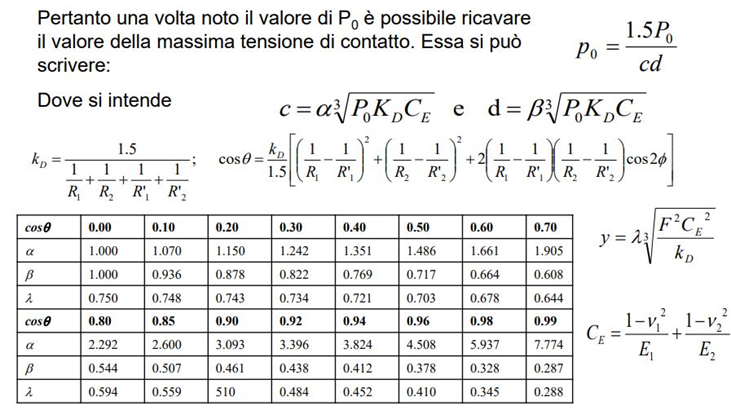
\includegraphics[width=0.5\linewidth]{immagini/screenshot017}
				\label{fig:screenshot017}
			\end{figure}
			\begin{figure}[H]
				\centering
				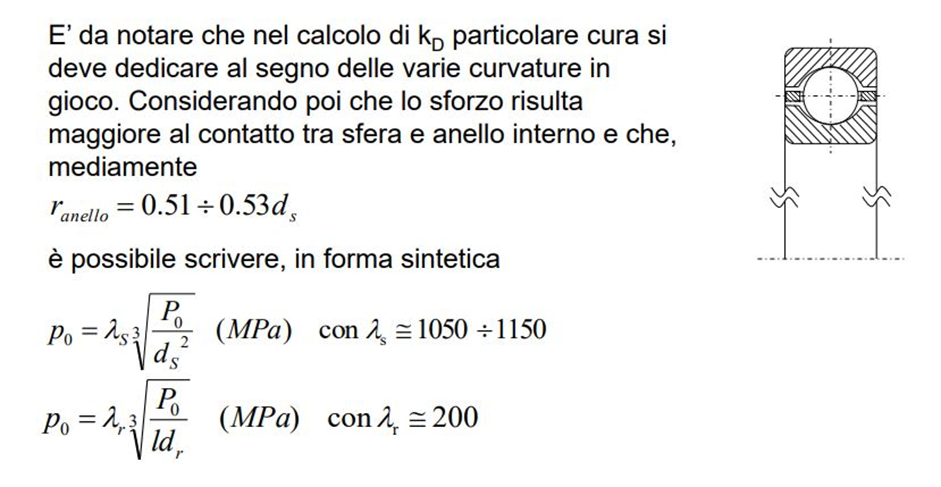
\includegraphics[width=0.5\linewidth]{immagini/screenshot018}
				\label{fig:screenshot018}
			\end{figure}
			Questa rappresenterebbe l’equivalente di una verifica statica del cuscinetto, cioè mi permette di ricavare la massima tensione hertziana da confrontare con l’ammissibile hertziana del materiale. \newline 
			
			Questo è solo il primo passo di un corretto dimensionamento del cuscinetto perché il fatto che il cuscinetto supporti forti carichi massimi è la condizione base, in realtà io devo garantire un funzionamento nel tempo del cuscinetto 
			
			Questi carichi variabili nel tempo portano a fenomeni di fatica perché localmente abbiamo una sfera che soggetta ad un campo di velocità fa un rotolamento senza strisciamento sulla sua sede e quindi avremo una componente di spostamento, di traslazione della sfera sulla guida più il rotolamento dovuto ad un campo di velocità a farfalla. \newline 
			
			Questo vuol dire che ciascun elemento della sfera subisce una condizione di compressione seguita da rilascio e così via a seconda della posizione in cui si trova
			
			\begin{figure}[H]
				\centering
				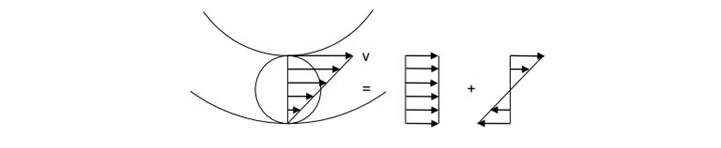
\includegraphics[width=0.5\linewidth]{immagini/screenshot019}
				\label{fig:screenshot019}
			\end{figure}
			
			\subsection{Verifica a fatica}
			L’approccio di fatica ad un cuscinetto viene fatto a livello globale del cuscinetto. \newline
			
			Il carico $C$ che troviamo in tutti i cataloghi di cuscinetti rappresenta il carico di riferimento al ginocchio della curva di Wöhler quindi associato a $10^6$ cicli. 
			
			Il coefficiente $m$ indica la pendenza della curva di Wöhler, convenzionalmente in mancanza di specifiche fornite dal produttore viene scelto pari a 3 per i cuscinetti a sfere e pari a 10/3 per i cuscinetti a rulli
			\begin{figure}[H]
				\centering
				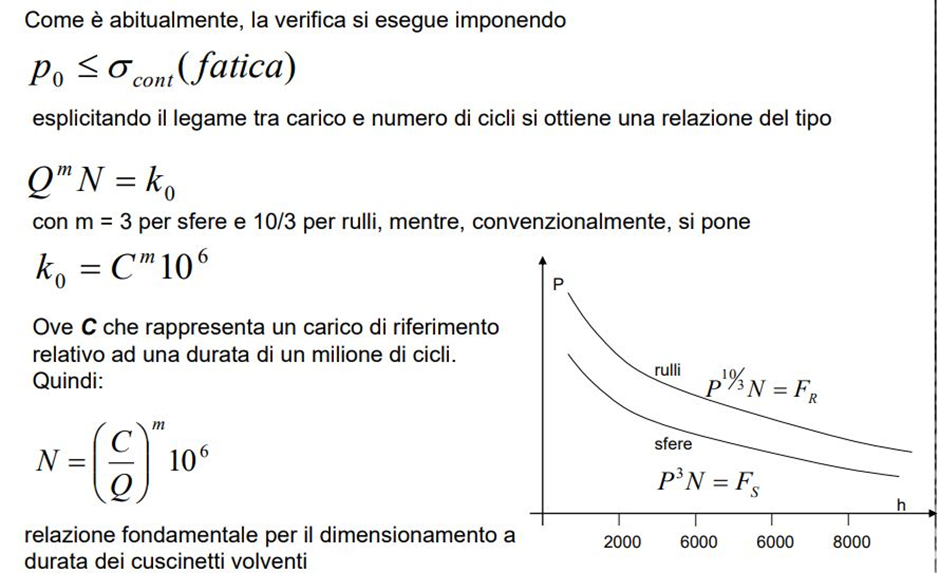
\includegraphics[width=0.5\linewidth]{immagini/screenshot020}
				\label{fig:screenshot020}
			\end{figure}
			Quindi data $C$ la resistenza a fatica del cuscinetto in esame, dato $Q$ il carico che mi viene fuori dal dimensionamento dell’albero (carico statico che si scarica sul cuscinetto) sono in grado di dire qual è il numero di cicli $N$ di applicazione del carico che può essere tradotto in ore di lavoro se conosco la velocità di lavorazione dell’albero. \newline
			
			Dovrò correggere questa durata in funzione delle condizioni al contorno, prima fra tutte la lubrificazione. 
			
			\subsubsection{Sistemi di lubrificazione}
			La lubrificazione può essere realizzata con grasso, olio lubrificante\dots
			
			La presenza di impurità nel lubrificante abbatte la durata del cuscinetto. \newline 
			
			Di solito i cuscinetti volventi non hanno una lubrificazione dedicata cioè non c’è un circuito di lubrificazione che manda l’olio all’interno del cuscinetto, ma di solito si hanno o delle tenute intorno al cuscinetto che intrappolano il lubrificante all’interno del cuscinetto oppure molto più spesso il cuscinetto pesca olio e lubrificante all’interno della cassa. \newline 
			
			Per non mettere a contatto la cassa con l’albero gli devo garantire un minimo di gioco radiale, è da lì che potranno entrare impurità e potrà uscire il lubrificante: devo impedire questo in qualche modo.
			E allora dovrò mettere dei materiali deformabili che possono strisciare sull’albero, oppure dovrò prevedere sistemi di scanalature o labirinti. 
			
			\subsubsection{Durata corretta}
			Abbiamo ragionato con un carico radiale $Q$ in realtà i cuscinetti possono sopportare anche carico assiale, quindi nella legge di durata a fatica dovrò correggere il carico $Q$ con un carico $P$ equivalente frutto del peso dei fattori $X$ e $Y$ forniti dai cataloghi in base al rapporto $\dfrac{F_A}{F_R}$.
			\[P = XF_R + YF_A\]
			\begin{figure}[H]
				\centering
				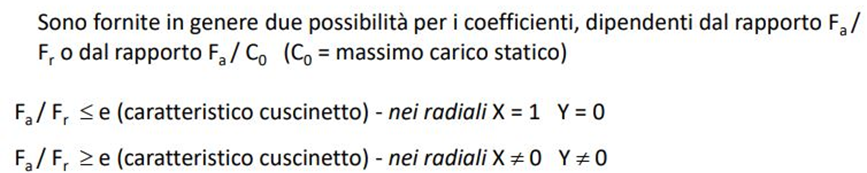
\includegraphics[width=0.5\linewidth]{immagini/screenshot021}
				\label{fig:screenshot021}
			\end{figure}
			Per quanto riguarda la durata del cuscinetto, oltre a mettere il termine $P$, dobbiamo aggiungere dei coefficienti correttivi che tengano conto della lubrificazione, delle impurità e anche dell’affidabilità del calcolo.\newline 
			
			Dovrò anche introdurre un coefficiente correttivo sull’affidabilità: il fenomeno della fatica è un fenomeno probabilistico e quindi se voglio un’affidabilità specifica sposterò la curva di Wohler più in alto o più in basso il che vuol dire aumentare o diminuire il numero di cicli. \newline 
			
			La legge corretta diventa quella riportata di seguito espressa in numero di ore (rispetto alla precedente si è diviso per 60 per trasformare in ore) e in funzione di due coefficienti $a_1$ e $a_{23}$. 
			
			\[L_h = \left(\dfrac{C}{Q}\right)^m\dfrac{10^6}{60n}a_1a_{23}\]
			
			Il coefficiente $a_1$ è il coefficiente di affidabilità, la curva di Wöhler di solito è espressa al 90\% di probabilità di sopravvivenza quindi $a_1$ vale 1 se voglio il 90\%\dots
			
			Il coefficiente $a_{23}$ dipende dalla viscosità. 
			\begin{figure}[H]
				\centering
				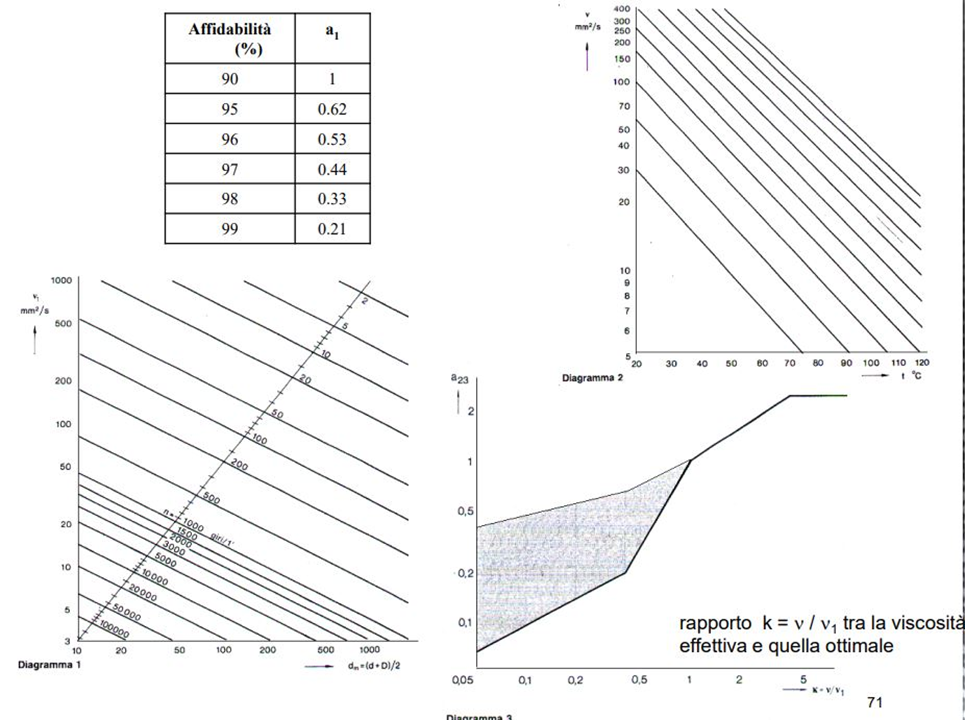
\includegraphics[width=0.7\linewidth]{immagini/screenshot022}
				\label{fig:screenshot022}
			\end{figure}
			L’andamento di questo coefficiente è riportato nel "diagramma 3" ed è espresso in funzione di un rapporto tra la viscosità effettiva e quella ottimale, il cui valore lo si ricava nel "diagramma 1" in funzione del numero di giri del cuscinetto e in funzione del diametro medio del cuscinetto.
			
			Per quanto riguarda invece la viscosità effettiva questa sarà data da una determinata curva alla quale è associato uno specifico lubrificante all'interno del "diagramma 2". 
			
			Il lubrificante si classifico in base alla sua viscosità a 40$^\circ$: una volta noto il lubrificante mi muovo lungo la curva e in base alla temperatura a cui effettivamente lavora il lubrificante leggo sulle ordinate il valore della viscosità effettiva. \newline
			
			\begin{center}
				\textbf{Il processo di scelta di un cuscinetto quindi non può che essere anche esso un procedimento iterativo.}
			\end{center}
			
			\subsection{Verifiche finali}
			Un’altra verifica da dover fare è quella legata alla velocità di rotazione: input del mio sistema.
			
			
			Il cuscinetto avrà delle velocità massime di lavoro che può sopportare così come le ha il lubrificante, dovrò quindi verificare che ci sia compatibilità. \newline 
			
			C’è poi un carico statico equivalente da dover confrontare in funzione delle $X$ e $Y$ tra il carico radiale e il carico assiale, confronto che viene fatto con delle $X$ e $Y$ proprie della prova statica, e il limite sarà sempre un $C_0$ tabellato nei cataloghi dei cuscinetti. \newline 
			
			Tutto ciò che abbiamo imparato a fare nell’ambito della fatica su un generico componente meccanico si può riportare sui cuscinetti.
			E allora così come un componente non sarà caricato sempre allo stesso di tensione lo stesso vale per il cuscinetto che non lavorerà sempre alle medesime condizioni di carico, possiamo fare anche per il cuscinetto un ragionamento di equivalenza alla Palmgren-Miner cioè andando a considerare che il cuscinetto sia sottoposto a un unico ciclo di carico equivalente che porti un danneggiamento a fatica pari alla sommatoria dei danneggiamenti associati ai singoli cicli di carico.
			\begin{figure}[H]
				\centering
				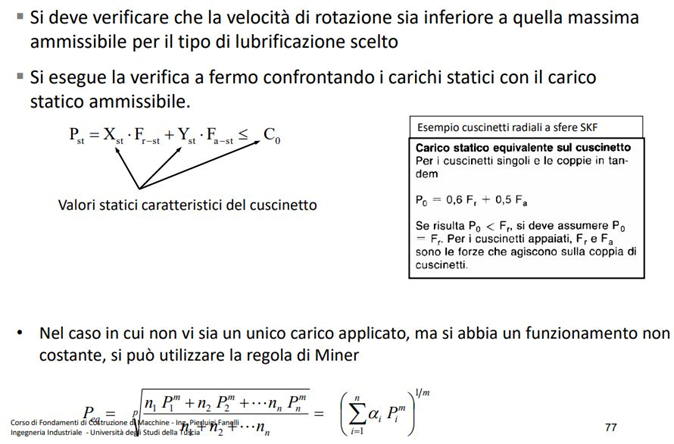
\includegraphics[width=0.5\linewidth]{immagini/screenshot023}
				\label{fig:screenshot023}
			\end{figure}
			
			
					
		\end{document}
		
	
		
		
